\chapter{Architecture de l’ISO bootable }
\minitoc

\clearpage
\section{Introduction}

Après avoir terminé la construction du système, nous devons fournir à l’utilisateur une image ISO bootable, qu’il pourra installer sur sa machine locale, que ce soit dans une machine virtuelle ou directement sur un matériel physique.

Le processus de génération de l’image ISO est aussi complexe que la construction du système elle-même. Il est donc nécessaire de bien comprendre le processus de démarrage.

\begin{figure}[H]
  \centering
  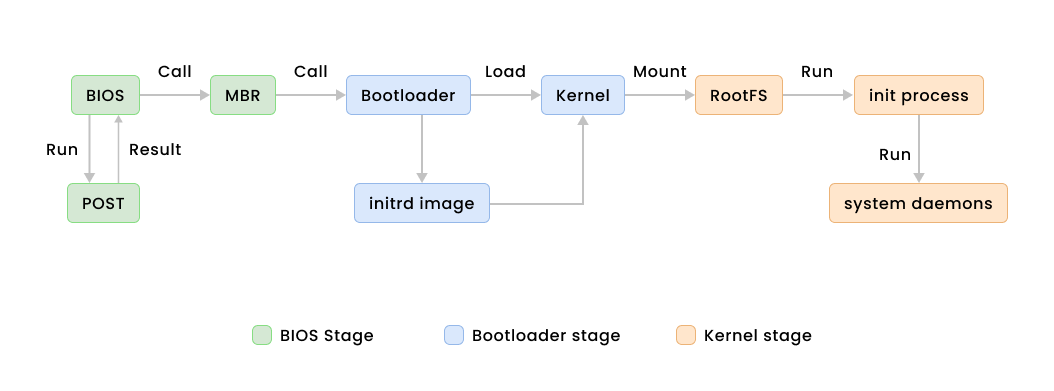
\includegraphics[width=1\textwidth, height=10cm]{images_pfe/bootloader process.png}
  \caption{Processus de démarrage de Kraken OS}
  \label{fig:kbootproc}
\end{figure}





\section{Démarrage du système}  
Lorsque vous appuyez sur le bouton d’alimentation du PC, un signal électrique déclenche le \textbf{POST} (\emph{Power-On Self-Test}), qui initialise le périphérique de démarrage (BIOS ou UEFI).  
\begin{itemize}  
  \item \textbf{Implication pour l’ISO} : L’ISO doit supporter \textbf{les modes BIOS et UEFI}.  
\end{itemize}  

\section{Rôle du chargeur d’amorçage}  
Le BIOS/UEFI charge le chargeur d’amorçage en lisant le fichier de configuration \texttt{isolinux.cfg}.  
\begin{itemize}  
  \item \textbf{Choix technique} : Nous utilisons \textbf{syslinux}, un chargeur d’amorçage léger.  
  \item \textbf{Fonctionnalités} :  
    \begin{itemize}  
      \item Chargement du noyau Linux (\texttt{vmlinuz}) et du disque RAM initial (\texttt{initrd}).  
      
    \end{itemize}  
\end{itemize}  

\section{Initrd personnalisé}  
L’\texttt{initrd} (disque RAM initial) fournit un ensemble minimal d’outils, de pilotes et d’utilitaires pour monter le système de fichiers racine.  
\begin{itemize}  
  \item \textbf{Choix technique} : Nous utilisons un \textbf{BusyBox personnalisé} pour générer l’\texttt{initrd}.  
  \item \textbf{Composants critiques} :  
    \begin{itemize}  
      \item \textbf{Le script \texttt{init}} :  
            Ce script doit être développé avec soin. Son objectif est de :  
            \begin{itemize}  
              \item Monter le système de fichiers \texttt{squashfs} (contenu de l’ISO),  
              \item Monter les systèmes de fichiers virtuels (\texttt{/proc}, \texttt{/sys}),  
              \item Basculer de l’environnement live ISO vers la racine (\texttt{chroot}) du système \texttt{squashfs}.  
            \end{itemize}  
      \item \textbf{Compilation de BusyBox} :  
            BusyBox est une suite logicielle qui regroupe plusieurs utilitaires Unix dans un seul fichier exécutable , dans notre cas BusyBox doit être compilé depuit le source a avec le support des fonctionnalités critiques, par exemple :  
            \begin{itemize}  
              \item Modules noyau : \texttt{loop}, \texttt{squashfs}, \texttt{overlayfs},  
                
            \end{itemize}  
    \end{itemize}  
\end{itemize}  

\begin{figure}[H]
  \centering
  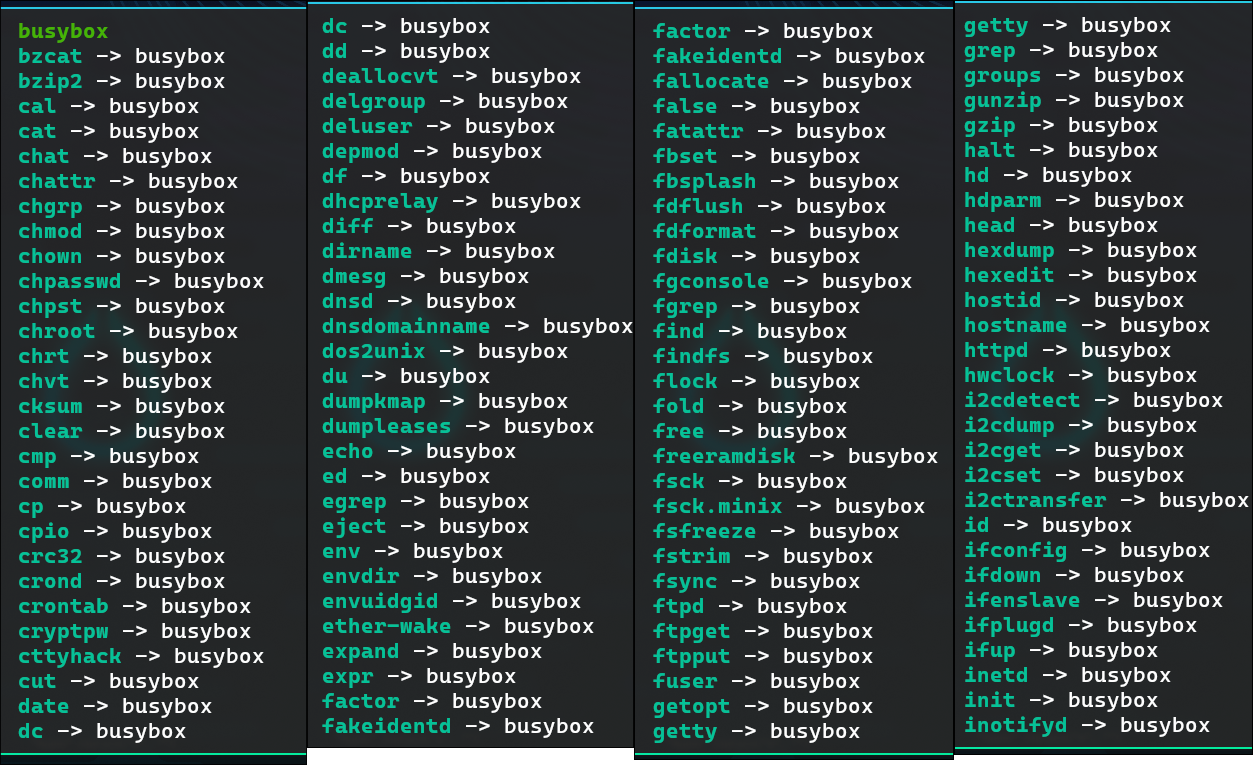
\includegraphics[width=1\textwidth, height=10cm]{images_pfe/busyboxbinary.png}
  \caption{structure de busybox executable}
  \label{fig:busybox}
\end{figure}
\clearpage
\section{Montage du système de fichiers racine}  
Le noyau monte le \textbf{rootfs} (système de fichiers racine).  
\begin{itemize}  
  \item \textbf{Choix technique} :  
    \begin{itemize}  
    \item Nettoyage des fichiers temporaires et du cache . 
      \item  Le système de fichiers racine doit être encapsulé dans une image \texttt{squashfs}, un format compressé en lecture seule optimisé pour les médias amorçables. 
       
        
    \end{itemize}  
\end{itemize}  

\section{Processus d’initialisation}  
Après le montage du \texttt{rootfs}, le noyau exécute \texttt{/sbin/init} (PID 1), qui lance les scripts SystemV.  
\begin{itemize}  
  \item \textbf{Séquence} :  
    \begin{enumerate}  
      \item Démarrage des démons (réseau, services système).  
      \item Affichage de l’écran de connexion graphique ( dans notre cas SDDM).  
    \end{enumerate}  
\end{itemize}  

\section{Environnement live et installation}  
L’ISO fonctionne d’abord en mode \textbf{live} pour installer dans un disque locale il faut developper :  
\begin{itemize}  
  \item \textbf{Interface graphique} :  une application dédiée guide l’utilisateur pour installer notre distibution sur le disque dur.  
  
   
\end{itemize}  




\section{Conclusion}
Dans ce chapitre nous avons détaillé les choix techniques et l'architecture du fichier iso bootable.\\
Dans le chapitre suivant, nous nous aborderons le processus de développement et d'implémentations, en détaillant les étapes de construction et les tests effectués sur la distribution.